\section{Uniform sampling}
\label{sec:uniform_sampling}

\begin{figure*}
    \centering
    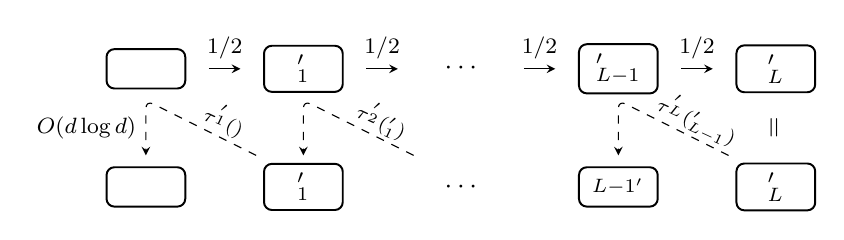
\begin{tikzpicture}
    % Matrices and sampling arrows
    \node [rectangle, line width = 0.25mm, draw, minimum width = 1cm, minimum height = .5cm, rounded corners = 0.1cm]
        (r) at (0,0) {$\A$};

    \draw [-stealth]
        (.8, 0) -- (1.2, 0) node[midway,above] {\footnotesize $1/2$};

    \node [rectangle, line width = 0.25mm, draw, minimum width = 1cm, minimum height = .5cm, rounded corners = 0.1cm]
        (r) at (2,0) {$\A_1'$};

    \draw [-stealth]
        (2.8, 0) -- (3.2, 0) node[midway,above] {\footnotesize $1/2$};
    \node []
        (r) at (4, 0) {$ \cdots $};
    \draw [-stealth]
        (4.8, 0) -- (5.2, 0) node[midway,above] {\footnotesize $1/2$};
    \node [rectangle, line width = 0.25mm, draw, minimum width = 1cm, minimum height = .5cm, rounded corners = 0.1cm]
        (r) at (6,0) {$\A_{L-1}'$};

    \draw [-stealth]
        (6.8, 0) -- (7.2, 0) node[midway,above] {\footnotesize $1/2$};
    \node [rectangle, line width = 0.25mm, draw, minimum width = 1cm, minimum height = .5cm, rounded corners = 0.1cm]
        (r) at (8,0) {$\A_L'$};

    \node [rectangle, line width = 0.25mm, draw, minimum width = 1cm, minimum height = .5cm, rounded corners = 0.1cm]
        (r) at (0,-1.5) {$\B$};

    \node [rectangle, line width = 0.25mm, draw, minimum width = 1cm, minimum height = .5cm, rounded corners = 0.1cm]
        (r) at (2,-1.5) {$\B_1'$};

    \node []
        (r) at (4, -1.5) {$ \cdots $};
    \node [rectangle, line width = 0.25mm, draw, minimum width = 1cm, minimum height = .5cm, rounded corners = 0.1cm]
        (r) at (6,-1.5) {$\B_{L-1'}$};

    \node [rectangle, line width = 0.25mm, draw, minimum width = 1cm, minimum height = .5cm, rounded corners = 0.1cm]
        (r) at (8,-1.5) {$\B_L'$};

    \node [rotate=90]
        (r) at (8, -.75) {$ = $};



    \draw [-stealth, rounded corners = 0.1cm, dashed]
        (1.4, -1.1) -- (0, -.4) -- (0, -1.1) node[midway, left, align=left] {\footnotesize $O(d\log d)$};
    \node [rotate=-25]
        (r) at (1, -.65) {\scriptsize $ \boldsymbol {\tau}^{\B_1'}(\A) $};

    \draw [-stealth, rounded corners = 0.1cm, dashed]
        (3.4, -1.1) -- (2, -.4) -- (2, -1.1) node[midway, left, align=left] {};
    \node [rotate=-25]
        (r) at (3, -.65) {\scriptsize $ \boldsymbol {\tau}^{\B_2'}(\A_1') $};

    \draw [-stealth, rounded corners = 0.1cm, dashed]
        (7.4, -1.1) -- (6, -.4) -- (6, -1.1) node[midway, left, align=left] {};
    \node [rotate=-25]
        (r) at (7, -.65) {\scriptsize $ \boldsymbol {\tau}^{\B_L'}(\A_{L-1}') $};
\end{tikzpicture}
    \caption{Structure of the recursive calls to \textsc{Approximate}. The
    leverage score vector $\bs \tau$ is indeed not explicitely computed, but is
    used for Grover search. The resulting matrix is $\bs B \approx_2 \bs A$.}
    \label{fig:sampling}
\end{figure*}

Uniform sampling does not uses $(R,k)$-reductions \textit{i.e.,}
Johnson-Lindenstrauss random projections as depicted in
\cite{li_iterative_2013}, and thus preserves the input matrix sparsity pattern,
which is usefull especially in the graph case. This will allow us, in this case,
to compute the leverage score of a single row in $O(1)$ quantum queries.

In our setting, computing leverages scores according to an approximation
$\bs{\tilde A}$ of the input matrix $\A$ requires to sample $$c \log d \sum_i
\tilde \tau_i$$ rows for a fixed constant $c$, where the $\tilde \tau_i$ are
computed according to $\bs{\tilde A}$.

In order to prove correctness of the algorithm we expose, it is convenient to
repesent the sampling of a matrix through the product with a diagonal matrix,
that we define below.

\begin{definition}
    Let  \emph{\texttt{Sample($\bs \tau, \alpha$)}} be a procedure that returns a
    diagonal matrix $S$ with independently chosen entries, and such $S_{ii} =
    p_i^{-1/2}$ with probability $p_i$ and $0$ otherwise, where $p_i = \min\{1,
    \alpha c \tau_i \log d\}$ for a fixed constant $c$.
\end{definition}

In the quantum setting, this is implemented by the procedure \textsc{Sample}
shown in \autoref{alg:sample}, thus there is no need to explicitly construct the
output matrix of the procedure. Nevertheless, it is necessary to show that the
two representations are equivalent.

\begin{theoremEnd}{claim}
    Given a matrix $\A$, on one hand let $\bs{S} = $ \emph{\texttt{Sample}}$(\bs 1,
    O(m/n))$ and consider $\bs{SA}$; on the other hand, let $\bs{A'}$ be a
    uniform ramdom subset of $O(m)$ rows of $\A$. Sampling according to
    $\bs{\tau^{SA}}$ is equivalent to sampling according to $\bs{\tau^{A'}}$.
\end{theoremEnd}

\begin{proofEnd}
A convient definition to consider is the one of the pseudoinverse of a vector.
\begin{definition}[Pseudoinverse of a vector]\label{def:vector-pseudoinverse}
   Let $x$ be a vector, the pseudoinverse of $x$ is
   $$
   x^+ = \begin{cases}
    \bs 0^T & \text{, if } x = \bs 0 \, ;\\
    \frac{x^*}{x^*x} & \text{, otherwise.}
   \end{cases}
   $$
\end{definition}

For the uniform sampling step, we consider $\bs S$ a sampling matrix with
$s_{ii} = 1$ \textit{w.p.} $\frac{m}{n}$ and $0$ otherwise. If $s_{ii} = 0$,
then $(sa_{i})^T$, the $i$-th row of $\bs{SA}$ is $\bs 0^T$, thus
$(sa_{i})^{T+}$ is $\bs 0$ : we can simply \emph{remove} this row since it does
not infere in the calculation of $\big((\bs{SA})^T\bs{SA}\big)^+$ according to
\autoref{def:vector-pseudoinverse}. Removing all the rows of $\A$ where $s_{ii}
= 0$ yields exactly $\bs{A'}$.
\end{proofEnd}
As long as the leverage score approximates used to sample are \textit{upper
bounds} on the true leverage score, \textit{i.e.,} for all $i$, $\tilde\tau_i
\geq \tau_i$, sampling $\A$ according to them yields a constant-factor spectral
approximation \cite{li_iterative_2013}.

\begin{theorem}[\cite{cohen_uniform_2014}]
    \label{thm:sum-expectation}
    Let $\A \in \mathbb R^{n\times d}$. Sampling uniformly at random $O(m)$ rows
    from $\A$ to form $\bs{\tilde A}$, implies, supposing one computes $\{\tilde \tau
    _i\}$ thanks to $\bs{\tilde A}$, that
    $$
    \mathbb E \left [ \sum_i \tilde \tau_i\right ] \leq \frac{nd}{m} \, .
    $$
\end{theorem}

The above theorem enables us to conclude on the number of rows to be sampled
given $m$.

\begin{theorem} [\cite{cohen_uniform_2014}]
    \label{thm:epsilon_spectral_approximation}
    Let $\A \in \mathbb R^{n\times d}$ suppose we sample uniformly $O(m)$ rows
    to form $\bs{A'}$. Computing $\tilde \tau_i = \min \{1,
    \tau_i^{\bs{A'}}(\A)\}$ and sampling $\A$ accordingly returns with high
    probability a constant factor spectral approximation of $\A$ with at most $O(\frac{nd\log
    d}{m})$ rows.
\end{theorem}

% and $\bs S = $ \emph{\texttt{Sample($\bs 1, \alpha$)}}.


Thus \autoref{thm:epsilon_spectral_approximation} implies correctness of
\autoref{alg:repeated-halving}.


\begin{algorithm}[H]
    \caption{\textsc{Approximate}($\bs A$)}
    \label{alg:repeated-halving}
    \begin{algorithmic}[1]
        \Ensure $\bs A \in \mathbb R ^{n \times d}$
        \State \textit{$\bs{A'} \<$ uniformly sample $\frac{n}{2}$ rows of $\bs A$}
        \If{$\bs{A'}$ \textit{ has more than $O(d\log d)$ rows }}
            \State $\bs{B'} \<$ \textsc{Approximate}($\bs{A'}$)
        \Else
            \State $\bs{B'} \< \bs {A'}$
        \EndIf
        % \State \textit{Set $\bs \tau = \Big\{ \tilde \tau_i = \min\{1, \tau_i^{\bs{A'}}(A)\} \Big\}_{i=1}^n$ }
        % \State \textit{Sample $\bs A$ according to $\bs \tau$ to form $\tilde A$}
        \State $\bs{B} \< $\textsc{Sample}$(\bs A, \bs B', O(d \log d))$
        \State \Return $\bs{B}$
    \end{algorithmic}
\end{algorithm}
Indeed, sampling $O(d \log d)$ rows is enough to obtain a constant factor
approximation: letting $m = O(n/2)$ in \autoref{thm:sum-expectation} yields
\begin{equation*}
\mathbbm E \left[ {\sum_i \tilde \tau_i} \right] = O(d) \, ,
\end{equation*}
hence
\begin{equation*}
    \log d \sum_i \tilde \tau_i = O(d \log d) \, .
\end{equation*}
The resulting matrix has $O(d\log d)$ rows and there are $O\big(\log
(\frac{n}{d\log d})\big)$ recursive calls to \textsc{Approximate}. It is
important to note that $\B$ is a
constant-factor-approximation of the matrix $\bs A$, which we write
$$\bs A \approx_{O(1)} \textsc{Approximate}(\bs A) \, .$$

\autoref{fig:sampling} shows graphically how the recursive sampling works.

It is possible to further speed up the calculation of leverage score by using
Johnson-Lindenstrauss transfom on each $\B_l'$, for all $1 \leq l \leq L$.

\subsection{Johnson-Lindenstrauss tranform}

For the sake of completeness, the Johnson-Lindenstrauss lemma is recalled in
\autoref{ap:jllemma}.

\subsubsection{Leverage score as a squared norm}

Let $\A \in \mathbb R^{n \times d}$, and recall that, for $a_i^T$ the $i$-th row
of $\A$, its leverage score $\tau_i$ is defined in \autoref{def:leverage-score}
as
$$
    \tau_i = a_i^T(\A^T\A)^+a_i \, .
$$
In order to express $\tau_i$ as a squared norm, let us denote
\begin{equation}\label{eq:def-xi}
    \bs \x_i := \A(\A^T\A)^+ a_i \, ,
\end{equation}
which yields the following proposition:
\begin{theoremEnd}{proposition}\label{prop:lv-as-norm}
    Given $\A$ an input matrix, one can compute the leverage scores of $\A$'s rows
    as follows:
    $$
        \tau_i(\A) = \|\bs \x_i \|_2^2 \, .
    $$
\end{theoremEnd}

\begin{proofEnd}
   Considering \autoref{eq:def-xi} yields
   \begin{equation*}
    \begin{aligned}
        \|\bs \x_i \|_2^2
            & = a_i^T \big((\A^T\A)^+\big)^T \A^T\A (\A^T\A)^+ a_i \\
            & = a_i^T \big((\A^T\A)^T\big)^+ \A^T\A (\A^T\A)^+ a_i \\
            & = a_i^T (\A^T\A)^+ \A^T\A (\A^T\A)^+ a_i \\
            & = a_i^T (\A^T\A)^+ a_i \\
            & = \tau_i(\A)
    \end{aligned}
   \end{equation*}
The second step comes from the commutation of the pseudoinversion with
transposition\footnote{$(\A^+)^T = (\A^T)^+$}, the third step follows
from the symmetry of $\A^T\A$, and the fourth step is the application of the
weak inverse property of pseudoinverses\footnote{$\A^+\A\A^+ = \A^+$}.
\end{proofEnd}


\subsubsection{Application of the JL transfom}

For our purpose, consider a matrix $\A \in \mathbb{R}^{\tilde O(d)\times d}$ and
let $\bs \x_i$ as introduced in \autoref{eq:def-xi}; thus, by
\autoref{prop:lv-as-norm}, $\|\bs \x_i\|_2^2 $ is exactly $ \tau_i$. Also, since
we can write $\Pi \bs \x_i = \Pi \A(\A^T\A)^+a_i$ with $\Pi \A(\A^T\A)^+ \in
\mathbb R^{\tilde O (\varepsilon^{-2})\times d}$, we denote $\| \Pi \bs \x_i
\|_2^2$ by $\hat \tau_i$. Thereby, we can restate \autoref{jl-lemma} as follows:

\begin{lemma}[DJL lemma, restated]
    For any $0 < \varepsilon < 1$, $\delta < 1/2$ and $d \in \mathbb N$, there
    exists a distribution over $\displaystyle \mathbb {R} ^{k\times d}$ from
    which the matrix $\Pi$ is drawn such that for $k =
    O\big(\varepsilon^{-2}\log(\delta^{-1})\big)$ and any vector $\x \in \mathbb
    R^d$, the following claim holds:
    \begin{equation*}
        \mathbb P \Big(\left | \hat \tau_i - \tau_i \right | > \varepsilon
        \cdot \tau_i \Big)<\delta \, .
    \end{equation*}
\end{lemma}

Let us denote by $X_i$ the event \guillemotleft $\left| \hat \tau_i - \tau_i
\right| > \varepsilon \cdot \tau_i$\guillemotright. Thus, taking the union
bound over all possible leverage scores, we have
\begin{equation*}
    \mathbb P (\bigcup_{i=1}^n X_i) \leq \sum_{i=1}^n \mathbb P(X_i) <
    \sum_{i=1}^n \delta = n \delta
\end{equation*}
Hence, setting $\delta = n^{-2}$ yields that, with probability $\geq 1-
\frac{1}{n}$, all leverage scores in the reduced space are an
$\varepsilon$-approximation of the original ones, \textit{i.e.,} for all $i \in [n]$,
\begin{equation}\label{eq:prob}
\left | \hat \tau_i - \tau_i \right | \leq  \varepsilon \cdot \tau_i \, .
\end{equation}


\begin{theoremEnd}{proposition}\label{prop:time-complexity-jl-lv}
    It is possible to compute a single leverage score in time $\hat
    O(\varepsilon^{-2}S)$, and such leverage score can be used to sample the
    input matrix and obtain a spectral approximation.
\end{theoremEnd}

\begin{proofEnd}
First, in order to have a more suitable expression of \autoref{eq:prob}, it is
convenient to break down the absolute value and examine both cases.
\begin{itemize}
    \item Case  $\hat \tau_i - \tau_i \leq 0$, then \textit{w.h.p.}
    \begin{table}[H]
        \centering
        \begin{tabular}{lrll}
        & $\hat \tau_i - \tau_i$ & $\geq$ & $- \varepsilon \cdot \tau_i$ \\
        $\Leftrightarrow$ & $\hat \tau_i$ & $\geq$ & $- \varepsilon \cdot \tau_i + \tau_i$ \\
        $\Leftrightarrow$ & $\hat \tau_i$ & $\geq$ & $(1 - \varepsilon) \cdot \tau_i$
        \end{tabular}
    \end{table}
    \item Case  $\hat \tau_i - \tau_i \geq 0$, then \textit{w.h.p.}
    \begin{table}[H]
        \centering
        \begin{tabular}{lrll}
            & $\hat \tau_i - \tau_i$ & $\leq$ & $\varepsilon \cdot \tau_i$ \\
            $\Leftrightarrow$ & $\hat \tau_i$ & $\leq$ & $\varepsilon \cdot \tau_i + \tau_i$ \\
            $\Leftrightarrow$ & $\hat \tau_i$ & $\leq$ & $(1 + \varepsilon) \cdot \tau_i$
        \end{tabular}
    \end{table}
\end{itemize}

Thus, still with probability $\geq 1 - \frac{1}{n}$, \autoref{eq:prob} can be
rephrased as follows,
$$
(1 - \varepsilon) \cdot \tau_i
    \; \leq \; \hat \tau_i
    \; \leq \; (1 + \varepsilon) \cdot \tau_i \, , \quad \forall i \in [n] \, .
$$
However, in order to obtain at the end a $\varepsilon$-spectral approximation
when sampling according to $\hat \tau_i$, it must hold that these approximations
are \textit{upper bounds} on the original ones. Note that here, what we denoted
by the \textit{original scores} are actually approximate of the \textit{true
scores}, \textit{i.e.,} the $\tilde\tau_i$. Thus, it suffices to sample
according to $\frac{1}{1-\varepsilon} \hat\tau_i$, since for all $i$, it holds
that
$$
\tilde \tau_i
    \; \leq \; \frac{1}{1-\varepsilon}\hat \tau_i
    \; \leq \; (\frac{1 + \varepsilon}{1-\varepsilon}) \tilde\tau_i \, ,
$$
which, by the way, implies that
$$
\mathbb E \left [\sum_{i=1}^n \tilde\tau_i \right ]
    \; \leq \; \mathbb E \left [\sum_{i=1}^n \frac{1}{1-\varepsilon}\hat \tau_i \right ]
    \; \leq \; \mathbb E \left [\sum_{i=1}^n \frac{1 + \varepsilon}{1-\varepsilon} \cdot \tilde\tau_i \right ] \, ,
$$
and equivalently, since the expectation of the sum of the approximate leverage
scores is bounded thanks to \autoref{thm:sum-expectation}, it holds that
$$
\frac{nd}{m}
    \; \leq \; \mathbb E \left [\sum_{i=1}^n \frac{1}{1-\varepsilon}\hat \tau_i \right ]
    \; \leq \; (\frac{1 + \varepsilon}{1-\varepsilon}) \frac{nd}{m} \, .
$$

Hence, it is possible to apply Johnson-Lindenstrauss transfrom to each
$\boldsymbol{B}_{l}'$ to get a matrix of dimension $\tilde O(\varepsilon^{-2})
\times d$, and thus computing a single leverage score in time $\tilde
O(\varepsilon^{-2}S)$.

\end{proofEnd}

\subsubsection{Time complexity of the scheme}\label{sec:time-complexity-jl}
Given as input a matrix $\A \in \mathbb{R}^{\tilde O(d) \times d}$, there is a
procedure with running time $\tilde O(d\varepsilon^{-2})$ that returns the
matrix $\Pi \in \mathbb R^{\tilde O(\varepsilon^{-2})\times \tilde O(d)}$ $-$
this procedure simply consists in setting each entry of $\Pi$ to independant
Gaussian random variable \cite{dasgupta_elementary_2003}. It takes time $\tilde
O (d^\omega)$ to obtain $\A(\A^T\A)^+$ and additional $\tilde
O(d^{2}\varepsilon^{-2})$ to compute the matrix-matrix product $\Pi
\A(\A^T\A)^+$. Thus, computing a single leverage score in time $\tilde
O(\varepsilon^{-2}S)$ requires a preprocessing time of $\tilde O(d^\omega)$. It
suffices to set $0 < \varepsilon < 1$ to be constant, so that each leverage
score requires time $\tilde O(S)$ to be computed. Doing so it holds, for any $0
\leq l \leq L$, that $\B'_l$ is still $O(1)$-spectral approximation of $\A'_l$
since the number of sampled rows stays unchanged and the leverage score used
remains upper bounds on the actual approximations, \emph{i.e.}, upper bounds on
the true leverage scores.

\subsection{Overall query complexity}
Let $L$ be the number of iterations required to obtain a matrix of $O(d\log d)$
rows. Thus, it holds that
$$
\frac{n}{2^L} = O(d \log d) \, ,
$$
hence, there is a total of
$$L = O(\log (\frac{n}{d \log d})) = \tilde O(1)$$
iterations.

Given a matrix $\A \in \mathbb{R}^{n \times d}$, let $S\leq d$ such that each
row of $\A$ has at most $S$ nonzero entries. Each call to \textsc{Sample}
computes $\tilde O(d)$ scores, where each score requires $O(S)$ queries. Since
each matrix has fewer than $n$ rows, the total number of rows of all of the
matrices together can be bounded by $Ln = \tilde O(n)$. Thus, by
\autoref{prop:quantum-queries-grover}, sampling $\tilde O(d)$ rows among $O(n)$
thoughout the $L$ iterations makes a total of $\tilde O(S\sqrt{nd})$ quantum
queries.

Furthermore, it is possible to store implicitly each reduced matrix, by
implicitly keeping track of the discarded rows through a string as shown in
\autoref{sec:data-structure-matrix}. However the last matrix has to be
explicitly written in order to compute $(\bs{A_L'}^T \bs{A_L'})^+$ : this
requires additional $\tilde{O}(dS)$ queries. Hence, the query complexity of
\autoref{alg:repeated-halving} is $\tilde{O} (S(\sqrt{nd} + d))$.

% Thus, there is a total of $\tilde O(d \log d \varepsilon^{-2})$ rows to be
% queried from the matrix while halving, among $O(n)$ rows, which requires $\tilde
% O(\sqrt{\frac{nd}{\varepsilon^2}})$ quantum queries thoughout Grover's
% iteration.